\section{Distillation-Assisted Network Tomography}
\label{sec:dist-qnt}

In this section, we develop a distillation-assisted tomography
protocol for the three-link star network.
\S\ref{subsec:direct-nt} first introduces direct pairwise
distillation and explains its identifiability limitation.
\S\ref{subsec:mergecast-nt} then presents a modified Mergecast
construction that provides estimation involving all three links.
\S\ref{subsec:Clifford-dressing} uses Clifford dressing to
obtain the additional estimation needed for complete estimation.
Finally, \S~\ref{linkpa} combines these measurement statistics
to construct JCE and MCE and establish the identifiability
of the three Pauli channels.
JCE requires the specified source-state fidelity condition
$F>1/2$, whereas MCE removes this requirement.

\subsection{Distillation-Assisted Unicast }
\label{subsec:direct-nt}



We begin with direct Unicast~\cite{Pirandola_2019} transmission between peripheral monitors,
where Unicast refers to single-path probe between one sender monitor and one receiver monitor (in the peripheral).
% where one monitor acts as the sender and the other as the
% receiver.
The three-link star network contains three two-link paths, each for
one pair of monitors as in Fig.~\ref{fig:three-link-star}. Consider the path
\(N_1\!-C\!-N_2\) shown in Fig.~\ref{fig:two-link-path}.
The Unicast procedure is as follows:
monitor \(N_1\) prepares a Bell pair \(\ket{\Phi^+}\), retains one qubit locally,
and sends the other to \(N_2\) through the Pauli channel \(\mathcal P_1\),
the central node \(C\), and the Pauli channel \(\mathcal P_2\).
The resulting state shared by monitor \(N_1\) and \(N_2\) is Bell diagonal,
as shown in Fig.~\ref{fig:two-link-path}.

\begin{figure}[tb]
    \centering
    \begin{tikzpicture}[
            line/.style={thick},
            proc/.style={
                    rectangle,
                    draw,
                    thick,
                    minimum width=0.7cm,
                    minimum height=0.55cm,
                    inner sep=1pt
                },
            endpoint/.style={
                    rectangle,
                    fill=blue,
                    draw=blue,
                    minimum size=0.18cm,
                    inner sep=0pt
                },
            station/.style={
                    rectangle,
                    draw,
                    dashed,
                    thick,
                    minimum width=0.55cm,
                    minimum height=0.55cm
                },
            center/.style={
                    circle,
                    fill=black,
                    draw=black,
                    minimum size=0.16cm,
                    inner sep=0pt
                },
            state/.style={
                    font=\scriptsize,
                    align=center
                }
        ]

        % Coordinates
        \coordinate (C)  at (0,0);
        \coordinate (A1) at (-3,0);
        \coordinate (A2) at (3,0);

        % Central node
        \node[center] (center) at (C) {};
        \node[station] at (C) {};
        \node[below=6pt] at (C) {$C$};

        % Peripheral node A1
        \node[endpoint] (node1) at (A1) {};
        \node[station] at (A1) {};
        \node[below=6pt] at (A1) {$N_1$};

        % Peripheral node A2
        \node[endpoint] (node2) at (A2) {};
        \node[station] at (A2) {};
        \node[below=6pt] at (A2) {$N_2$};

        % Pauli channels
        \node[proc] (P1) at (-1.5,0) {$\mathcal P_1$};
        \node[proc] (P2) at ( 1.5,0) {$\mathcal P_2$};

        % Transmission path
        \draw[line] (node1) -- (P1) -- (center);
        \draw[line] (center) -- (P2) -- (node2);

        % Initial Bell-state vector at A1
        \node[state] at (-3,-1.25) {
            $\displaystyle
                \begin{bmatrix}
                    1  \\
                    1  \\
                    -1 \\
                    1
                \end{bmatrix}$
        };

        % State after channel P1, arriving at C
        \node[state] at (0,-1.25) {
            $
                \begin{bmatrix}
                    1       \\
                    q_{X1}  \\
                    -q_{Y1} \\
                    q_{Z1}
                \end{bmatrix}$
        };

        % State after channels P1 and P2, arriving at A2
        \node[state] at (3,-1.25) {
            $
                \begin{bmatrix}
                    1             \\
                    q_{X1}q_{X2}  \\
                    -q_{Y1}q_{Y2} \\
                    q_{Z1}q_{Z2}
                \end{bmatrix}$
        };

    \end{tikzpicture}

    \caption{
        Two-link path \(N_1\!-\!C\!-\!N_2\) through the central node \(C\).
        The column vectors below the nodes are the restricted
        Pauli--Liouville representation of the shared state at the
        corresponding transmission stage.
        By symmetry, the same protocol can be applied to the other
        two two-link paths, \(N_1- C- N_3\) and
        \(N_2- C- N_3\).
    }
    \label{fig:two-link-path}
\end{figure}
Applying the same procedure along the all three paths, including the other two \(N_2 \!-\!C\!-\!N_3\) and \(N_1\!-\!C\!-\!N_3\), gives the quantum states with restricted Pauli--Liouville representations as follows,
\begin{equation}
    \begin{aligned}
        \plket{\rho_{12}}
         & =
        \begin{bmatrix}
            1               &
            q_{X,1}q_{X,2}  &
            -q_{Y,1}q_{Y,2} &
            q_{Z,1}q_{Z,2}
        \end{bmatrix}^{T}, \\
        \plket{\rho_{13}}
         & =
        \begin{bmatrix}
            1               &
            q_{X,1}q_{X,3}  &
            -q_{Y,1}q_{Y,3} &
            q_{Z,1}q_{Z,3}
        \end{bmatrix}^{T}, \\
        \plket{\rho_{23}}
         & =
        \begin{bmatrix}
            1               &
            q_{X,2}q_{X,3}  &
            -q_{Y,2}q_{Y,3} &
            q_{Z,2}q_{Z,3}
        \end{bmatrix}^{T}.
    \end{aligned}
    \label{eq:direct-two-link-states}
\end{equation}

For each path, the two monitors independently generate three copies
of the shared state via the Unicast transmission above and then perform the double-selection protocol in~\S\ref{subsec:doub}.

Whenever the source state for distillation in~\eqref{eq:direct-two-link-states} satisfies the fidelity condition of
Lemma~\ref{lem:double-selection-statistics},
the double-selection
statistics in~\eqref{eq:double-selection-probabilities} \emph{uniquely estimate} its nontrivial Pauli correlations (e.g., the last three entries of \(\plket{\rho_{12}}\):
\(\widehat{q_{X,1}q_{X,2}}\),
\(\widehat{q_{Y,1}q_{Y,2}}\)
and \(\widehat{q_{Z,1}q_{Z,2}}\)). Thus, applying this
procedure to all three paths estimate any \(\widehat{q_{P, \ell}q_{P,\ell'}}\)
for any \(P\in\{X,Y,Z\}\)
and \((\ell, \ell') \in \{(1,2), (1,3), (2,3)\}\).


% \begin{equation}
%     q_{P,1}q_{P,2},
%     \quad
%     q_{P,1}q_{P,3},
%     \quad
%     q_{P,2}q_{P,3},
%     \quad P\in\{X,Y,Z\}.
% \end{equation}

% Insert Fig.~\ref{fig:two-link-path} here.

\paragraph{Identifiability challenge}

For each $P\in\{X,Y,Z\}$, the double-selection statistics yield
estimates of the pairwise products
$q_{P,1}q_{P,2}$, $q_{P,1}q_{P,3}$, and $q_{P,2}q_{P,3}$,
each involving an even number of factors.
From these three estimates, one can, for instance, estimate
the parameter $q_{P,1}$ as
$\pm\sqrt{
        \frac{
            \widehat{q_{P,1}q_{P,2}} \times \widehat{q_{P,1}q_{P,3}}
        }{
            \widehat{q_{P,2}q_{P,3}}
        }
    }$, with a sign ambiguity.
That is, there are two possible sign choices for each Pauli component,
across all three components giving up to eight choices in total.
This ambiguity suggests that this protocol alone cannot uniquely
identify all channels.


To resolve this sign ambiguity, we introduce a
Mergecast protocol in the following subsection,
which  generates estimates involving
all three links (i.e., products of an odd number of factors).
By combining the estimates with the ones in Unicast, we resolve
this sign ambiguity and uniquely estimate the channel parameters.

% In this scheme, only $\rho_{12}$ and $\rho_{13}$ are generated
% by direct transmission.
% For the remaining path $N_2\!-\!C\!-\!N_3$, we instead use
% undressed and Clifford-dressed Mergecast configurations,

% Instead, our protocol
% directly generates only \(\rho_{12}\) and \(\rho_{13}\).
% For the remaining path \(N_2\!-\!C\!-\!N_3\), we replace direct
% transmission with undressed and Clifford-dressed modified Mergecast
% configurations. 






\subsection{Distillation-Assisted Mergecast}
\label{subsec:mergecast-nt}
Fig.~\ref{fig:modified-mergecast} illustrates the Mergecast
protocol~\cite{wang2025quantumnetworktomographygeneral},
which introduces correlations involving all three links
to resolve the sign ambiguity.
We apply this protocol to the path $N_2\!-\!C\!-\!N_3$
and then use the double-selection protocol to estimate
the resulting Bell-diagonal state.
\begin{figure*}[tb]
    \centering
    \begin{tikzpicture}[
            x=1cm,
            y=1cm,
            font=\small,
            wire/.style={thick},
            region/.style={
                    draw,
                    dashed,
                    thick,
                    rounded corners=4pt,
                    fill=blue!20
                },
            gate/.style={
                    draw,
                    thick,
                    fill=white,
                    minimum width=0.7cm,
                    minimum height=0.45cm,
                    inner sep=3pt
                },
            distillation/.style={
                    draw,
                    thick,
                    rounded corners=4pt,
                    fill=orange!18,
                    minimum width=1.8cm,
                    minimum height=0.8cm,
                    align=center
                },
            boundary/.style={draw=red,dashed,thick},
            state/.style={
                    anchor=north,
                    font=\small,
                    inner sep=0pt
                },
            ent/.style={
                    thick,
                    decorate,
                    decoration={
                            snake,
                            amplitude=0.55mm,
                            segment length=1.4mm
                        }
                }
        ]

        % Preparation regions and central node.
        \draw[region] (-0.15,0.65) rectangle (0.85,1.35);
        \draw[region] (-0.15,-0.35) rectangle (0.85,0.35);
        \draw[region] (5.10,-0.35) rectangle (6.80,1.35);

        % Auxiliary qubit from N_1 through P_1.
        \draw[wire] (0.35,1.00) -- (6.30,1.00);
        \node[gate,rounded corners=6pt]
        at (0.35,1.00) {$\ket{0}$};
        \node[gate] at (3.00,1.00) {$\mathcal P_1$};

        % Bell pair prepared at N_2.
        \draw[wire] (-0.05,0.00) -- (0.10,0.00);
        \draw[ent] (0.10,0.00) -- (0.60,0.00);
        \filldraw[draw=black,fill=white,thick]
        (0.10,0.00) circle (0.045);
        \filldraw[draw=black,fill=white,thick]
        (0.60,0.00) circle (0.045);
        \node[font=\scriptsize] at (0.35,-0.22)
        {$\ket{\Phi^+}$};

        % Traveling Bell qubit.
        \draw[wire] (0.60,0.00) -- (11.10,0.00);
        \node[gate] at (3.00,0.00) {$\mathcal P_2$};
        \node[gate] at (9.00,0.00) {$\mathcal P_3$};

        % CNOT at C: auxiliary control, traveling Bell qubit target.
        \fill (5.65,1.00) circle (2.2pt);
        \draw[thick] (5.65,1.00) -- (5.65,0.00);
        \draw[thick] (5.65,0.00) circle (0.105);
        \draw[thick] (5.65,-0.105) -- (5.65,0.105);
        \draw[thick] (5.545,0.00) -- (5.755,0.00);

        % Discard the auxiliary qubit.
        \draw[thick,->] (6.30,1.00) -- (6.30,0.48);
        \node[font=\scriptsize] at (6.30,0.28) {discard};

        % Node labels.
        \node at (0.35,1.65) {$N_1$};
        \node at (0.35,-0.60) {$N_2$};
        \node at (5.95,-0.60) {$C$};

        % Transmission slices.
        \foreach \x/\stage in {1.5/1,4.5/2,7.5/3,10.5/4}{
                \draw[boundary] (\x,-0.85) -- (\x,1.45);
                \node at (\x,1.65) {$\stage$};
            }

        % Bell-pair vectors in the ordered basis (II,XX,YY,ZZ).
        \node[state] at (1.5,-1.05) {
            $\begin{bmatrix}
                    1  \\
                    1  \\
                    -1 \\
                    1
                \end{bmatrix}$
        };

        \node[state] at (4.5,-1.05) {
            $\begin{bmatrix}
                    1        \\
                    q_{X,2}  \\
                    -q_{Y,2} \\
                    q_{Z,2}
                \end{bmatrix}$
        };

        \node[state] at (7.5,-1.05) {
            $\begin{bmatrix}
                    1               \\
                    q_{X,2}         \\
                    -q_{Z,1}q_{Y,2} \\
                    q_{Z,1}q_{Z,2}
                \end{bmatrix}$
        };

        \node[state] at (10.5,-1.05) {
            $\begin{bmatrix}
                    1                      \\
                    q_{X,2}q_{X,3}         \\
                    -q_{Z,1}q_{Y,2}q_{Y,3} \\
                    q_{Z,1}q_{Z,2}q_{Z,3}
                \end{bmatrix}$
        };

        % Three independent preparations supply the distillation input.
        \node[font=\scriptsize,align=center] at (11.75,0.90)
        {Repeat preparation\\three times};

        \node[distillation] (DS) at (13.15,0.00)
        {Double\\selection};

        \draw[wire,->] (11.10,0.00) -- (DS.west)
        node[midway,above=4pt,font=\scriptsize]
        {$\bigl(\rho_{\text{m,}23}\bigr)^{\otimes3}$};

        \node[font=\scriptsize,below=6pt] at (DS.south)
        {$N_2\leftrightarrow N_3$ (LOCC)};

        % Conditionally retained output pair.
        \draw[wire,->] (DS.east) -- (15.35,0.00)
        node[midway,above=4pt,font=\scriptsize]
        {$\rho_{\text{m},23}^{\mathrm{out}}$};

    \end{tikzpicture}

    \caption{
        Mergecast preparation followed by double-selection protocol.
        Slices 1--4 illustrate the entanglement-generation procedure, adapted
        from the Mergecast protocol in
        \cite{wang2025quantumnetworktomographygeneral}.
        The column vectors give the restricted Pauli--Liouville
        representations of the reduced two-qubit state.
        The preparation is repeated independently three times, after which
        monitors \(N_2\) and \(N_3\) perform double-selection protocol to
        distill a retained entangled pair and estimate the input-state
        parameters from the measurement statistics.
    }
    \label{fig:modified-mergecast}
\end{figure*}
The procedure is as follows.
\begin{enumerate}
    \item Node \(N_2\) prepares \(\ket{\Phi^+}\), retains one qubit,
          and sends the other to \(C\) through \(\mathcal P_2\). Meanwhile,
          \(N_1\) sends an auxiliary qubit in \(\ket{0}\) to \(C\) through
          \(\mathcal P_1\).

    \item Node \(C\) applies a CNOT with the auxiliary qubit as the
          control and the Bell-pair qubit as the target. It then traces out (i.e., discard)
          the control and forwards the target to \(N_3\) through
          \(\mathcal P_3\).
    \item After generating three independent copies from repeating steps 1) and 2), node \(N_2\) and
          \(N_3\) perform double-selection protocol.
\end{enumerate}

Before distillation, each source state shared by \(N_2\) and \(N_3\) is
\begin{equation}
    \plket{\rho_{\text{m},23}}
    =
    \begin{bmatrix}
        1                      &
        q_{X,2}q_{X,3}         &
        -q_{Z,1}q_{Y,2}q_{Y,3} &
        q_{Z,1}q_{Z,2}q_{Z,3}
    \end{bmatrix}^{ T}.
    \label{eq:mergecast-undressed-state}
\end{equation}


By Lemma~\ref{lem:double-selection-statistics}, the double-selection
statistics yield estimates of the nontrivial Pauli coefficients
of $\rho_{\text{m},23}$.
For example, combining the resulting estimate of
$q_{Z,1}q_{Z,2}q_{Z,3}$ with the previously obtained estimate
of $q_{Z,1}q_{Z,2}$ gives
\(
\widehat{q}_{Z,3}
\coloneqq
\frac{
    \widehat{q_{Z,1}q_{Z,2}q_{Z,3}}
}{
    \widehat{q_{Z,1}q_{Z,2}}
},
\)
This illustrates how combining the estimates from the two protocols
resolves the sign ambiguity.
Further details are presented in \S~\ref{linkpa}.

% The double-selection statistics determine the three-link correlation
% \(q_{Z,1}q_{Z,2}q_{Z,3}\). Combining it with the pairwise correlations
% obtained from direct distillation gives
% \begin{equation}
% \begin{aligned}
%     q_{Z,1}
%     &=
%     \frac{
%         (q_{Z,1}q_{Z,2})(q_{Z,1}q_{Z,3})
%     }{
%         q_{Z,1}q_{Z,2}q_{Z,3}
%     },\\
%     q_{Z,2}
%     &=
%     \frac{
%         q_{Z,1}q_{Z,2}q_{Z,3}
%     }{
%         q_{Z,1}q_{Z,3}
%     },\\
%     q_{Z,3}
%     &=
%     \frac{
%         q_{Z,1}q_{Z,2}q_{Z,3}
%     }{
%         q_{Z,1}q_{Z,2}
%     }.
% \end{aligned}
% \end{equation}

To recover the remaining parameters
\(q_{X,\ell}\) and \(q_{Y,\ell}\), we need to access correlations
in other Pauli bases. We achieve this through channel dressing,
as described below.


\begin{remark}[Fidelity inefficiency of the Mergecast protocol]
    Although this Mergecast operation may
    reduce the fidelity of the final source state in~\eqref{eq:mergecast-undressed-state} shared by node \(N_2\) and \(N_3\), it
    provides information that cannot be obtained from Unicast and resolve the sign ambiguity issue.
    In other words, it trades some end-to-end
    fidelity for the identifiability.
\end{remark}

\subsection{Clifford-Dressed Pauli Channels}
\label{subsec:Clifford-dressing}

We adapt the channel-dressing technique of Wang et al.~\cite{wang2025quantumnetworktomographygeneral} to the
Mergecast protocol.
Specifically, in Fig.~\ref{fig:modified-mergecast},
we apply different Clifford
dressings to \(\mathcal P_2\) and \(\mathcal P_3\), while leaving
\(\mathcal P_1\) unchanged.
Dressing the channels is equivalent to change
    input and output bases of the channels, providing the statistics for estimating other channel parameters.



The dressing uses the Hadamard gate \(H\) and phase gate \(S\).
Both are Clifford gates, which bijectively map Pauli operators to Pauli
operators up to a sign under
conjugation~\cite{Gottesman1998Heisenberg}.
Ignoring signs, \(H\) exchanges \(X\) and \(Z\), while \(S\)
exchanges \(X\) and \(Y\). Together, these exchanges generate all
permutations of \(\{X,Y,Z\}\).
When a Pauli channel is dressed by a Clifford gate and its Hermitian conjugate,
the signs cancel, so the dressing simply permutes its PTM
eigenvalues. We use the Clifford gates \(SHS\) and \(S\) to define
\begin{equation}
\begin{aligned}
\mathcal P_2^{(SHS)}
\coloneqq SHS\circ\mathcal P_2\circ(SHS)^\dagger,\
\mathcal P_3^{(S)}
&\coloneqq S\circ\mathcal P_3\circ S^\dagger.
\end{aligned}
\label{eq:dressed-pauli-channels}
\end{equation}
These dressings exchange the \(Y\) and \(Z\) eigenvalues of
\(\mathcal P_2\), and the \(X\) and \(Y\) eigenvalues of
\(\mathcal P_3\), respectively, as illustrated in
Fig.~\ref{fig:pauli-channel-dressing}.

\begin{figure}[tb]
    \centering
    \resizebox{\columnwidth}{!}{%
        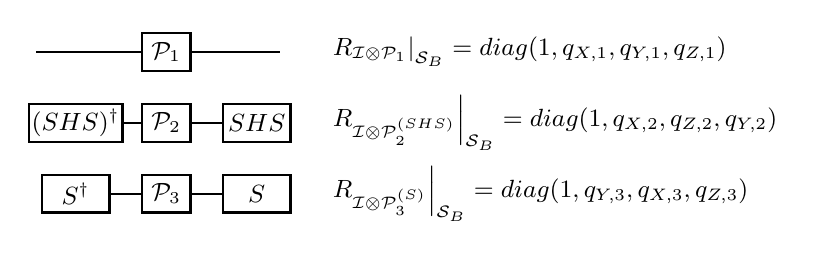
\begin{tikzpicture}[
                x=1cm,
                y=1cm,
                font=\small,
                wire/.style={draw=black,thick},
                gate/.style={
                        draw=black,
                        thick,
                        fill=white,
                        minimum width=0.62cm,
                        minimum height=0.48cm,
                        inner sep=1pt
                    },
                widegate/.style={gate,minimum width=0.86cm}
            ]

            % Link 1 remains undressed.
            \draw[wire,-] (0.15,1.25) -- (3.25,1.25);
            \node[gate] at (1.80,1.25) {$\mathcal P_1$};
            \node[anchor=west] at (3.75,1.25) {
                $\left.R_{\mathcal I\otimes\mathcal P_1}\right|_{\mathcal S_B}
                    =\operatorname{diag}(1,q_{X,1},q_{Y,1},q_{Z,1})$
            };

            % Apply (SHS)^\dagger before P_2 and SHS after P_2.
            \draw[wire,-] (0.15,0.35) -- (3.25,0.35);
            \node[widegate] at (0.65,0.35) {$(SHS)^\dagger$};
            \node[gate] at (1.80,0.35) {$\mathcal P_2$};
            \node[widegate] at (2.95,0.35) {$SHS$};
            \node[anchor=west] at (3.75,0.35) {
                $\left.R_{\mathcal I\otimes\mathcal P_2^{(SHS)}}\right|_{\mathcal S_B}
                    =\operatorname{diag}(1,q_{X,2},q_{Z,2},q_{Y,2})$
            };

            % Apply S^\dagger before P_3 and S after P_3.
            \draw[wire,-] (0.35,-0.55) -- (3.25,-0.55);
            \node[widegate] at (0.65,-0.55) {$S^\dagger$};
            \node[gate] at (1.80,-0.55) {$\mathcal P_3$};
            \node[widegate] at (2.95,-0.55) {$S$};
            \node[anchor=west] at (3.75,-0.55) {
                $\left.R_{\mathcal I\otimes\mathcal P_3^{(S)}}\right|_{\mathcal S_B}
                    =\operatorname{diag}(1,q_{Y,3},q_{X,3},q_{Z,3})$
            };

        \end{tikzpicture}%
    }
    \caption{
        Link-dependent Clifford dressing used in the modified Mergecast
        protocol.
        Each channel $\mathcal P_\ell$ is preceded by $U_\ell^\dagger$
        and followed by $U_\ell$, with $U_1=I$, $U_2=SHS$, and $U_3=S$.
        Thus, $\mathcal P_1$ remains unchanged, while the PTM eigenvalues
        of $\mathcal P_2$ and $\mathcal P_3$ are permuted as
        $(q_{X,2},q_{Y,2},q_{Z,2})
            \mapsto(q_{X,2},q_{Z,2},q_{Y,2})$
        and
        $(q_{X,3},q_{Y,3},q_{Z,3})
            \mapsto(q_{Y,3},q_{X,3},q_{Z,3})$, respectively.
        These dressings allow the Mergecast protocol to access the
        mixed products $q_{Z,1}q_{Z,2}q_{X,3}$ and
        $q_{Z,1}q_{Y,2}q_{Z,3}$, which provide the additional information
        needed to resolve the remaining sign ambiguities.
    }
    \label{fig:pauli-channel-dressing}
\end{figure}

Replacing \(\mathcal P_2\) and \(\mathcal P_3\) with these dressed
channels in the Mergecast-based distillation protocol produces
\begin{equation}
    \plket{\rho_{\text{d},23}}
    =
    \begin{bmatrix}
        1                      &
        q_{X,2}q_{Y,3}         &
        -q_{Z,1}q_{Z,2}q_{X,3} &
        q_{Z,1}q_{Y,2}q_{Z,3}
    \end{bmatrix}^{\mathsf T}.
    \label{eq:mergecast-dressed-state}
\end{equation}
By Lemma~\ref{lem:double-selection-statistics}, the double-selection
statistics  recovers the
nontrivial Pauli coefficients of \(\rho_{\text{d},23}\).
In particular, the last two coefficients provide the information
needed to determine \(q_{X,3}\) and \(q_{Y,2}\).
Together with the direct and undressed Mergecast measurements,
they enable the complete channel estimation described next.

\subsection{Link-Parameter Estimation}
\label{linkpa}
\paragraph{Joint-Coincidence Estimator (JCE)}
Under Assumption~\ref{ass:fidelity-condition} on source-state fidelity, JCE combines the estimates obtained from the four configurations
to estimate the individual channel parameters.


By Lemma~\ref{lem:double-selection-statistics}, the double-selection
statistics of the directly generated states $\rho_{12}$ and
$\rho_{13}$ yield estimators $\widehat{\pi}_{12}^{(P)}$ and
$\widehat{\pi}_{13}^{(P)}$ of the pairwise products defined as follows,
\begin{equation}
    \begin{aligned}
        \pi_{12}^{(P)}
         & \coloneqq q_{P,1}q_{P,2},\,
        \pi_{13}^{(P)}
        \coloneqq q_{P,1}q_{P,3},
        \, P\in\{X,Y,Z\}.
    \end{aligned}
    \label{eq:direct-correlations}
\end{equation}
Similarly, the double-selection statistics of the undressed
Mergecast state $\rho_{\text{m},23}$ yield an estimator
$\widehat{\tau}_Z$ of the three-link correlation
\[
    \tau_Z\coloneqq q_{Z,1}q_{Z,2}q_{Z,3}.
\]
Combining these estimates, we define
\begin{equation}
    \begin{aligned}
        \widehat{q}_{Z,1}
        \coloneqq
        \frac{\widehat{\pi}_{12}^{(Z)}
            \widehat{\pi}_{13}^{(Z)}}{\widehat{\tau}_Z},
        \widehat{q}_{Z,2}
        \coloneqq
        \frac{\widehat{\tau}_Z}{\widehat{\pi}_{13}^{(Z)}},
        \widehat{q}_{Z,3}
        \coloneqq
        \frac{\widehat{\tau}_Z}{\widehat{\pi}_{12}^{(Z)}}.
    \end{aligned}
    \label{eq:z-parameter-reconstruction}
\end{equation}

To estimate the remaining parameters, we use the double-selection
statistics of the dressed Mergecast state $\rho_{\text{d},23}$.
These statistics yield estimators $\widehat{\mu}_X$ and
$\widehat{\mu}_Y$ of
\[
    \mu_X\coloneqq q_{Z,1}q_{Z,2}q_{X,3},
    \qquad
    \mu_Y\coloneqq q_{Z,1}q_{Y,2}q_{Z,3}.
\]
Dividing these estimates by the corresponding  estimates gives
\begin{equation}
    \widehat{q}_{X,3}
    \coloneqq
    \frac{\widehat{\mu}_X}{\widehat{\pi}_{12}^{(Z)}},
    \qquad
    \widehat{q}_{Y,2}
    \coloneqq
    \frac{\widehat{\mu}_Y}{\widehat{\pi}_{13}^{(Z)}}.
    \label{eq:reference-parameter-reconstruction}
\end{equation}
These expressions provide estimates of both the magnitude and sign
of one parameter in each of the $X$ and $Y$ sectors.
The remaining parameters are then estimated sequentially as
\begin{equation}
    \begin{aligned}
        \widehat{q}_{X,1}
         & \coloneqq
        \frac{\widehat{\pi}_{13}^{(X)}}{\widehat{q}_{X,3}},
         &
        \widehat{q}_{X,2}
         & \coloneqq
        \frac{\widehat{\pi}_{12}^{(X)}}{\widehat{q}_{X,1}}, \\
        \widehat{q}_{Y,1}
         & \coloneqq
        \frac{\widehat{\pi}_{12}^{(Y)}}{\widehat{q}_{Y,2}},
         &
        \widehat{q}_{Y,3}
         & \coloneqq
        \frac{\widehat{\pi}_{13}^{(Y)}}{\widehat{q}_{Y,1}}.
    \end{aligned}
    \label{eq:remaining-parameter-reconstruction}
\end{equation}

Finally, applying the transformation in
Lemma~\ref{lem:bell-pauli-transformation} gives estimators
of the Pauli-error probabilities of each channel:
\begin{equation}
    \begin{bmatrix}
        \widehat{A}_\ell \\
        \widehat{B}_\ell \\
        \widehat{C}_\ell \\
        \widehat{D}_\ell
    \end{bmatrix}
    \coloneqq
    W^{ T}
    \begin{bmatrix}
        1                     \\
        \widehat{q}_{X,\ell}  \\
        -\widehat{q}_{Y,\ell} \\
        \widehat{q}_{Z,\ell}
    \end{bmatrix},
    \qquad \ell\in\{1,2,3\}.
    \label{eq:channel-probability-reconstruction}
\end{equation}

To summarize, ~\eqref{eq:z-parameter-reconstruction}--%
\eqref{eq:remaining-parameter-reconstruction} give estimates
of the link parameters, while~\eqref{eq:channel-probability-reconstruction} gives the
corresponding estimates of the Pauli-error probabilities.
The corresponding exact estimation establishes the
following identifiability result.

\begin{theorem}[Estimation with a fidelity assumption]
\label{cor:three-link-identifiability}
Under Assumptions~\ref{ass:nonzero-eigenvalues}
and~\ref{ass:fidelity-condition}, all nine link-level PTM
eigenvalues, and hence all three Pauli channels, are uniquely
identifiable from double-selection statistics through
~\eqref{eq:z-parameter-reconstruction}--%
\eqref{eq:remaining-parameter-reconstruction}, by combining
the Unicast{} and Mergecast{} protocols with link-dependent
Clifford dressing.
\end{theorem}

The fidelity assumption can be relaxed when estimating
$q_{Z,1}$, $q_{Z,2}$, and $q_{Z,3}$, as follows.

\begin{observation}[Estimation of the link parameters $q_{Z,\ell}$]
\label{obs:z-link-reconstruction}
The exact
$Z$-basis coincidence probabilities obtained from
$\rho_{12}$, $\rho_{13}$, and $\rho_{\text{m,}23}$ uniquely
determine $q_{Z,1}$, $q_{Z,2}$, and $q_{Z,3}$ without
Assumption~\ref{ass:fidelity-condition}.
The corresponding estimators are given by~\eqref{eq:z-parameter-reconstruction}.
\end{observation}

Indeed, Observation~\ref{lem3} allows the products
$q_{Z,1}q_{Z,2}$, $q_{Z,1}q_{Z,3}$, and
$q_{Z,1}q_{Z,2}q_{Z,3}$ to be estimated from the
corresponding $Z$-basis measurement statistics alone.
These products suffice to estimate all three $q_{Z,\ell}$.

\paragraph{Marginal-Coincidence Estimator (MCE)}
Building on Observation~\ref{obs:z-link-reconstruction},
MCE removes the
fidelity requirement, constituting another key contribution of this work.
We retain~\eqref{eq:z-parameter-reconstruction} for
estimating $q_{Z,\ell}$ and extend the same estimation
to $q_{X,\ell}$ and $q_{Y,\ell}$ through uniform Clifford dressing.
This scheme uses only the $Z$-basis measurement statistics, leaving the other
information unused.

                                                                                                                                                                                                                                                                                                                                                                                                                                                                                                                                                                                                                                                                                                                                                                                                                                                                                                                                                                                                                                                                                                                                                                                                                                                                                                                                                                                                                                                                                                                                                                                                                                                                                                                                                                                                                                                                                                                                                                                                                                                                                                                                                                                                                                                                                                                                                                                                                                                                                                                                                                                                                                                                                                                                                                                                                                                                                                                                                                                                                                                                                                                                                                                                                                                                                                                                                                                                                                                                                                                                                                                                                                                                                                                                                                                                                                                                                                                                                                                                                                                                                                                                                                                                                                                                                                                                                                                                                                                                                                                                                                                                                                                                                                                                                                                                                                                                                                                                                                                                                                                                                                                                                                                                                                                                                                                                                                                                                                                                                                                                                                                                                                                                                                                                                                                                                                                                                                                                                                                                                                                                                                                            
                                                                                                                                                                                                                                                                                                                                                                                                                                                                                                                                                                                                                                                                                                                                                                                                                                                                                                                                                                                                                                                                                                                                                                                                                                                                                                                                                                                                                                                                                                                                                                                                                                                                                                                                                                                                                                                                                                                                                                                                                                                                                                                                                                                                                                                                                                                                                                                                                                                                                                                                                                                                                                                                                                                                                                                                                                                                                                                                                                                                                                                                                                                                                                                                                                                                                                                                                                                                                                                                                                                                                                                                                                                                                                                                                                                                                                                                                                                                                                                                                                                                                                                                                                                                                                                                                                                                                                                                                                                                                                                                                                                                                                                                                                                                                                                                                                                                                                                                                                                                                                                                                                                                                                                                                                                                                                                                                                                                                                                                                                                                                                                                                                                                                                                                                                                                                                                                                                                                                                                                                                                                                                                                 
\begin{figure}[tb]
    \centering
    \resizebox{\columnwidth}{!}{%
        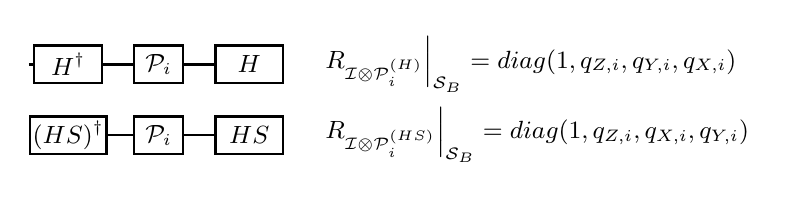
\begin{tikzpicture}[
                x=1cm,
                y=1cm,
                font=\small,
                wire/.style={draw=black,thick},
                gate/.style={
                        draw=black,
                        thick,
                        fill=white,
                        minimum width=0.62cm,
                        minimum height=0.48cm,
                        inner sep=1pt
                    },
                widegate/.style={gate,minimum width=0.86cm}
            ]

            % H dressing: the effective Z parameter is q_{X,i}.
            \draw[wire] (0.15,0.35) -- (3.25,0.35);
            \node[widegate] at (0.65,0.35) {$H^\dagger$};
            \node[gate] at (1.80,0.35) {$\mathcal P_i$};
            \node[widegate] at (2.95,0.35) {$H$};
            \node[anchor=west] at (3.75,0.35) {
                $\left.R_{\mathcal I\otimes\mathcal P_i^{(H)}}\right|_{\mathcal S_B}
                    =\operatorname{diag}(1,q_{Z,i},q_{Y,i},q_{X,i})$
            };

            % HS dressing: the effective Z parameter is q_{Y,i}.
            \draw[wire] (0.15,-0.55) -- (3.25,-0.55);
            \node[widegate] at (0.65,-0.55) {$(HS)^\dagger$};
            \node[gate] at (1.80,-0.55) {$\mathcal P_i$};
            \node[widegate] at (2.95,-0.55) {$HS$};
            \node[anchor=west] at (3.75,-0.55) {
                $\left.R_{\mathcal I\otimes\mathcal P_i^{(HS)}}\right|_{\mathcal S_B}
                    =\operatorname{diag}(1,q_{Z,i},q_{X,i},q_{Y,i})$
            };

        \end{tikzpicture}%
    }
    \caption{
        Clifford dressing of the Pauli channel $\mathcal P_i$ and the
        resulting permutations of its PTM eigenvalues.
        The upper and lower circuits implement the $H$ and $HS$
        dressings, respectively, with the corresponding restricted
        PTMs shown on the right.
        These dressings give $q_{Z,i}^{(H)}=q_{X,i}$ and
        $q_{Z,i}^{(HS)}=q_{Y,i}$, allowing the original $X$ and $Y$
        parameters to be estimated through the effective $Z$ parameter.
    }
    \label{fig:pauli-channel-dressing2}
\end{figure}

    To estimate $q_{X,\ell}$ and $q_{Y,\ell}$, we apply each of the
    Clifford dressings shown in Fig.~\ref{fig:pauli-channel-dressing2}
    uniformly to all three channels in the network.
    This differs from JCE, which applies different
    dressings to different channels in Mergecast.
    The $H$ and $HS$ dressings map $q_{X,\ell}$ and $q_{Y,\ell}$,
    respectively, to the effective $Z$ eigenvalues  of the dressed channels:
    \begin{equation}
        q_{Z,\ell}^{(H)}=q_{X,\ell},
        \qquad
        q_{Z,\ell}^{(HS)}=q_{Y,\ell},
        \qquad \forall \ell\in\{1,2,3\}.
    \end{equation}
For each dressing, we apply the same transformation to all
three links and repeat the Unicast{} and undressed Mergecast{}
procedures with the dressed channels.
Observation~\ref{lem3} then yields estimates
$\widehat{\pi}_{12}^{(P)}$, $\widehat{\pi}_{13}^{(P)}$, and
$\widehat{\tau}_P$ of $q_{P,1}q_{P,2}$, $q_{P,1}q_{P,3}$,
and $q_{P,1}q_{P,2}q_{P,3}$, respectively, for $P\in\{X,Y\}$.
Substituting these estimates into~\eqref{eq:z-parameter-reconstruction}, with $Z$ replaced
by $X$ or $Y$, gives
\begin{equation}
\begin{aligned}
    \widehat{q}_{X,1}
    &\coloneqq
    \frac{\widehat{\pi}_{12}^{(X)}
          \widehat{\pi}_{13}^{(X)}}{\widehat{\tau}_X},
    \quad
    \widehat{q}_{X,2}
    \coloneqq
    \frac{\widehat{\tau}_X}{\widehat{\pi}_{13}^{(X)}},
    \quad
    \widehat{q}_{X,3}
    \coloneqq
    \frac{\widehat{\tau}_X}{\widehat{\pi}_{12}^{(X)}},\\
    \widehat{q}_{Y,1}
    &\coloneqq
    \frac{\widehat{\pi}_{12}^{(Y)}
          \widehat{\pi}_{13}^{(Y)}}{\widehat{\tau}_Y},
    \quad
    \widehat{q}_{Y,2}
    \coloneqq
    \frac{\widehat{\tau}_Y}{\widehat{\pi}_{13}^{(Y)}},
    \quad
    \widehat{q}_{Y,3}
    \coloneqq
    \frac{\widehat{\tau}_Y}{\widehat{\pi}_{12}^{(Y)}}.
\end{aligned}
\label{eq22}
\end{equation}
Together with~\eqref{eq:z-parameter-reconstruction},
these estimators give the following estimation result.
\begin{theorem}[Estimation without a fidelity assumption]
        \label{thm:reconstruction-without-fidelity}
        Even without Assumption~\ref{ass:fidelity-condition}, all link-level
        PTM eigenvalues of these three Pauli channels in the star network remain uniquely
        identifiable from double-selection statistics  via~\eqref{eq:z-parameter-reconstruction} and~\eqref{eq22} by combining
        Clifford dressing with the Unicast and Mergecast protocols.
    \end{theorem}
\textcolor{blue}{
The two estimators establish identifiability under different conditions and exhibit a trade-off between measurement efficiency and applicability. JCE exploits joint $X/Z$ coincidence statistics and link-dependent Clifford dressing to estimate all nine channel parameters using four measurement configurations, but requires the source-state fidelity condition $F>1/2$. In contrast, MCE relies only on $Z$-basis coincidence statistics and uniform Clifford dressing, removing the fidelity requirement at the cost of increasing the number of configurations from four to nine. Consequently, each complete round requires 16 measured qubits for JCE and 36 for MCE. Thus, JCE is more resource-efficient in terms of configurations and measurements per round when the fidelity condition holds, whereas MCE offers broader applicability without this condition. The statistical efficiency of the two estimators under equal measurement budgets is further evaluated in \S~\ref{sec:problem-formulation}.}